\documentclass[14pt,a4paper]{extreport}
\usepackage[top=2cm, left=3cm, bottom=2cm, right=1cm]{geometry}
\usepackage[utf8x]{inputenc} % Включаем поддержку UTF8
\usepackage[russian]{babel} % Пакет поддержки русского языка
\usepackage{lscape}
\usepackage{fancyhdr}
\usepackage{textcase}
\usepackage{graphicx}
\usepackage{caption}
\usepackage{refstyle}
\usepackage{indentfirst}
\usepackage{hyperref}
\usepackage{listings}
\usepackage{xcolor}

\lstdefinestyle{sharpc}{language=[Sharp]C, frame=lr, rulecolor=\color{blue!80!black}}
\lstset{ %
language=[Sharp]C,                 % выбор языка для подсветки (здесь это С)
basicstyle=\small\sffamily, % размер и начертание шрифта для подсветки кода
numbers=left,               % где поставить нумерацию строк (слева\справа)
numberstyle=\tiny,           % размер шрифта для номеров строк
stepnumber=1,                   % размер шага между двумя номерами строк
numbersep=5pt,                % как далеко отстоят номера строк от подсвечиваемого кода
backgroundcolor=\color{white}, % цвет фона подсветки - используем \usepackage{color}
showspaces=false,            % показывать или нет пробелы специальными отступами
showstringspaces=false,      % показывать или нет пробелы в строках
showtabs=false,             % показывать или нет табуляцию в строках
frame=single,              % рисовать рамку вокруг кода
tabsize=2,                 % размер табуляции по умолчанию равен 2 пробелам
captionpos=t,              % позиция заголовка вверху [t] или внизу [b] 
breaklines=true,           % автоматически переносить строки (да\нет)
breakatwhitespace=false, % переносить строки только если есть пробел
escapeinside={\%*}{*)}   % если нужно добавить комментарии в коде
}

\title{}
\author{}

\begin{document}
%----------ТИТУЛЬНЫЙ-ЛИСТ--------------
	\center
	Министерство образования Республики Беларусь\\
	Учреждение образования «Белорусский государственный университет информатики и радиоэлектроники»
	\vspace*{2cm}
	\endcenter
	\raggedright
	Факультет компьютерных систем и сетей\\
	\medskip
	Кафедра программного обеспечения информационных технологий\\
	\medskip
	Дисциплина:  Компьютерные системы и сети (КСиС)
	\vspace*{2cm}
	\center
	ПОЯСНИТЕЛЬНАЯ ЗАПИСКА\\
	к курсовому проекту\\
	на тему\\
	\medskip
	Веб-сайт доска объявлений\\
	\medskip
	БГУИР КП  1-40 01 0 26 ПЗ
	\vspace*{4cm}
	\endcenter
	\raggedright
	\hspace*{7.94cm}Студент:  гр. 351002 Гучок О.А.\\
	\bigskip
	\hspace*{7.94cm}Руководитель: асс. Третьяков Ф.И.\\
	\center
	\vspace*{2cm}
	Минск 2015
	\pagestyle{empty}
%-------ЛИСТ-ЗАДАНИЯ--------------
	\newpage
	\center
	Учреждение образования\\
	\medskip
	«Белорусский государственный университет информатики и радиоэлектроники»\\
	\medskip
	Факультет компьютерных систем и сетей\\
	\medskip
	\endcenter
	\raggedright
	\hspace*{9.53cm}УТВЕРЖДАЮ\\
	\hspace*{9.53cm}Заведующий кафедрой ПОИТ\\
	\hspace*{9.53cm}\underline{\hspace{6cm}} \\
	\hspace*{11cm}\small (подпись) \normalsize\\
	\hspace*{9.53cm}\underline{\hspace{5cm}}2015 г.\\
	\medskip
	\center
	ЗАДАНИЕ\\
	по курсовому проектированию\\
	\medskip
	\endcenter
	\raggedright
	Студенту \underline{Гучку Олегу Анатольевичу}\\
	\begin{enumerate}
	\item Тема работы \underline{Веб-сайт доска объявлений}\\ 
	\item Срок сдачи студентом законченной работы \underline{DD.MM.YYYY}
	\item Исходные данные к работе \underline{Среда разработки Visual Studio 2013. }
	\item Содержание расчётно-пояснительной записки (перечень вопросов, которые подлежат разработке)\\
	\underline{\hspace*{16cm}}\hspace*{-16cm}Введение. 1. Анализ литературных источников. 2. Постановка задачи\\
	\underline{\hspace*{16cm}}\hspace*{-16cm}3.Разработка программного средства. 4. Руководство по \\
	\underline{\hspace*{16cm}}\hspace*{-16cm}использованию веб-сайта. Заключение. Приложения.
	\item Перечень графического материала (с точным обозначением обязательных чертежей и графиков)\\
	\underline{1. Схема алгоритма}
	\item Консультант по курсовой работе\\
	\underline{Третьяков Ф.И.}  
	\item Дата выдачи задания \underline{DD.MM.YYYY}
	\item Календарный график работы над проектом на весь период проектирования (с обозначением сроков выполнения и процентом от общего объёма работы):\\
	\underline{\hspace*{16cm}}\hspace*{-16cm}раздел 1 к DD.MM.YYYY – 15 \% готовности работы;\\  
	\underline{\hspace*{16cm}}\hspace*{-16cm}разделы 2, 3 к DD.MM.YYYY – 30 \% готовности работы;\\ 
	\underline{\hspace*{16cm}}\hspace*{-16cm}раздел 4 к DD.MM.YYYY – 60 \% готовности работы;\\
	\underline{\hspace*{16cm}}\hspace*{-16cm}раздел 5, 6 к DD.MM.YYYY  –  90 \% готовности работы;\\
	\underline{\hspace*{16cm}}\hspace*{-16cm}оформление пояснительной записки и графического материала к\\
	\underline{\hspace*{16cm}}\hspace*{-16cm}DD.MM.YYYY – 100 \% готовности работы.\\
	\underline{\hspace*{16cm}}\hspace*{-16cm}Защита курсового проекта с DD по DD декабря YYYY г.\\
	\end{enumerate}
	\hspace*{7cm}РУКОВОДИТЕЛЬ\underline{\hspace*{6cm}}\hspace*{-3.9cm}Третьяков Ф.И.\\
	\hspace*{11.5cm}\small (подпись) \normalsize\\
	\bigskip
	Задание принял к исполнению \underline{\hspace*{10.5cm}}\hspace*{-8cm}Гучок О.А. DD.MM.YYYYг.\\
	\hspace*{7cm}\small (дата и подпись студента) \normalsize\\
	%-------СОДЕРЖАНИЕ--------------
	\newpage
	\pagestyle{plain}
	%\renewcommand{\headrulewidth}{0px}
	%\fancypagestyle{plain}{\cfoot{}\rfoot{\thepage}}
	
	\renewcommand\contentsname{\center\normalsize \textbf{СОДЕРЖАНИЕ} \endcenter}
	\tableofcontents
	\endcenter
	%-----ВВЕДЕНИЕ-----
	\newpage
	\addcontentsline{toc}{section}{ВВЕДЕНИЕ}
	\section*{\center\normalsize ВВЕДЕНИЕ \endcenter}
	\hspace{4ex}
	
	\parindent = 1cmТехнологический прогресс и всемирная сеть способствовали зна­чительному увеличению объема информации, углублению и расширению наших представлений об окружающем мире. До сих пор основным способом предъявления полученных новых научных знаний была публикация научных
статей и разработок ученых. Гипермедиа ресурсы позволили осуществить
быстрый доступ ко всей научной информации, размещенной в Интернете.
Научные дискуссии, обмен мнениями и критическими замечаниями могут
быть реализованы в режиме реального времени, что, несомненно, способст­
вует более быстрому продвижению научных открытий в реальную жизнь.
Сфера интернет-технологий является одной из наиболее динамично разви­
вающихся направлений обработки информации. Технологии не успевают по­
лучить своего полного распространения, как их сменяют другие, более со­
вершенные. \par
	Бесчисленное множество новых технологий делает нашу жизнь невозможной без быстрого доступа к информации. В наше время очень легко получить информацию, одним из способов быстрого доступа к ней является сайт.\par
	Создание сайтов на сегодняшний день, становится одной из наиболее актуальных и востребованных услуг. Именно поэтому, большинство компаний уже оценили все преимущества такого предложения как создание сайтов и позаботились о разработке подходящего ресурса.\par
	Пользователю приятно посещать те Web-страницы, которые имеют стильное оформление, не отягощены чрезмерно графикой и анимацией, быстро загружаются и правильно отображаются в окне Web-браузера. Но может возникнуть и другая проблема - сайт может оказаться не интересным пользователю и та информация, которую он несет, окажется не востребованной. Именно поэтому важно, чтобы сайт отвечал всем требованиям пользователя.\par
	Актуальность данной работы заключается в том, что с учетом скорости развития сети Интернет и направления e-commerce, рынок WEB-разработки огромен и очень перспективен.\par
	Целью работы является формирование теоретических знаний по проектированию web-сайта и практических навыков по его разработке. Выбранная технология - ASP.NET MVC.\par
	Инфраструктура ASP.NET MVC Framework реализует шаблон MVC и при этом обеспечивает существенно улучшенное разделение ответственности. На самом деле в ASP.NET MVC внедрен современный вариант MVC, который особенно хорошо подходит для веб-приложений.\par
	Для хранения информации пользователя будет использоваться база данных, доступ к которой будет контролироваться самим приложением.\par	

	%-----АНАЛИТИЧЕСКИЙ ОБЗОР ЛИТЕРАТУРЫ----
	\newpage
	\addcontentsline{toc}{section}{1 АНАЛИТИЧЕСКИЙ ОБЗОР ЛИТЕРАТУРЫ}
	\addcontentsline{toc}{subsection}{1.1 Платформа .Net Framework}	
	\section*{\normalsize\hspace{4ex}1 АНАЛИТИЧЕСКИЙ ОБЗОР ЛИТЕРАТУРЫ}
	\textbf{1.1  Платформа .Net Framework}

	\parindent=1cm .NET Framework  - программная платформа, выпущенная компанией Microsoft в 2002 году. Основой платформы является общеязыковая среда исполнения Common Language Runtime (CLR), которая подходит для разных языков программирования. Функциональные возможности CLR доступны в любых языках программирования, использующих эту среду.\par
	Архитектура .NET.Программа для .NET Framework, написанная на любом поддерживаемом языке программирования, сначала переводится компилятором в единый для .NET промежуточный байт-код Common Intermediate Language (CIL) (ранее назывался Microsoft Intermediate Language, MSIL). В терминах .NET получается сборка, англ. assembly. Затем код либо исполняется виртуальной машиной Common Language Runtime (CLR), либо транслируется утилитой NGen.exe в исполняемый код для конкретного целевого процессора. Использование виртуальной машины предпочтительно, так как избавляет разработчиков от необходимости заботиться об особенностях аппаратной части. В случае использования виртуальной машины CLR, встроенный в неё JIT-компилятор «на лету» (just in time) преобразует промежуточный байт-код в машинные коды нужного процессора. Современная технология динамической компиляции позволяет достигнуть высокого уровня быстродействия. Виртуальная машина CLR также сама заботится о базовой безопасности, управлении памятью и системе исключений, избавляя разработчика от части работы. Архитектура .NET Framework описана и опубликована в спецификации Common Language Infrastructure (CLI), разработанной Microsoft и утверждённой ISO и ECMA. В CLI описаны типы данных .NET, формат метаданных о структуре программы, система исполнения байт-кода и многое другое.\par
	Объектные классы .NET, доступные для всех поддерживаемых языков программирования, содержатся в библиотеке Framework Class Library (FCL). В FCL входят классы Windows Forms, ADO.NET, ASP.NET, Language Integrated Query, Windows Presentation Foundation, Windows Communication Foundation и другие. Ядро FCL называется Base Class Library (BCL).
Для выполнения данной курсовой работы была использована среда разработки Microsoft Visual Studio 2012 Express. 
	Немного о самой среде разработки.\par
	Visual Studio включает в себя редактор исходного кода с поддержкой технологии IntelliSense и возможностью простейшего рефакторинга кода. Встроенный отладчик может работать как отладчик уровня исходного кода, так и как отладчик машинного уровня. Остальные встраиваемые инструменты включают в себя редактор форм для упрощения создания графического интерфейса приложения, веб-редактор, дизайнер классов и дизайнер схемы базы данных. Visual Studio позволяет создавать и подключать сторонние дополнения (плагины) для расширения функциональности практически на каждом уровне, включая добавление поддержки систем контроля версий исходного кода.\par
	~\\

	\addcontentsline{toc}{subsection}{1.2 Веб-технология ASP.NET}
	\textbf{1.2 Веб-технология ASP.NET}

	\parindent=1cm ASP.NET  - технология создания веб-приложений и веб-сервисов от компании Майкрософт. Она является составной частью платформы Microsoft .NET и развитием более старой технологии Microsoft ASP. На данный момент последней версией этой технологии является ASP.NET 4.5.\par
 	Хотя ASP.NET берёт своё название от старой технологии Microsoft ASP, она значительно от неё отличается. Microsoft полностью перестроила ASP.NET, основываясь на Common Language Runtime (CLR), которая является основой всех приложений Microsoft .NET. Разработчики могут писать код для ASP.NET, используя практически любые языки программирования, входящие в комплект .NET Framework (C\#, Visual Basic.NET и JScript .NET). ASP.NET имеет преимущество в скорости по сравнению со скриптовыми технологиями, так как при первом обращении код компилируется и помещается в специальный кэш, и впоследствии только исполняется, не требуя затрат времени на парсинг, оптимизацию, и т. д.\par
	Преимущества ASP.NET:\par
	• Компилируемый код выполняется быстрее, большинство ошибок отлавливается ещё на стадии разработки;\par
	• Значительно улучшенная обработка ошибок во время выполнения запущеной готовой программы, с использованием блоков try..catch;\par
	• Пользовательские элементы управления (controls) позволяют
выделять часто используемые шаблоны, такие как меню сайта;\par
	• Использование метафор, уже применяющихся в Windows-приложениях, например, таких как элементы управления и события;\par
	• Расширяемый набор элементов управления и библиотек классов позволяет быстрее разрабатывать приложения;\par
	• ASP.NET опирается на многоязыковые возможности .NET, что позволяет писать код страниц на VB.NET, Delphi.NET, Visual C\#, J\# и т. д;\par
	• Возможность кэширования всей страницы или её части для увеличения производительности;\par
	• Возможность кэширования данных, используемых на странице;\par
	• Возможность разделения визуальной части и бизнес-логики по разным файлам («code behind»);\par
	• Расширяемая модель обработки запросов;\par
	• Расширенная событийная модель;\par
	• Расширяемая модель серверных элементов управления;\par
	• Наличие master-страниц для задания шаблонов оформления страниц;\par
	• Поддержка CRUD-операций при работе с таблицами через GridView;\par
	• Встроенная поддержка AJAX.\par

	~\\

	\addcontentsline{toc}{subsection}{1.3 Реляционные базы данных}
	\textbf{1.3 Реляционные базы данных}

	\parindent=1cm База данных — это набор таблиц, состоящих из столбцов и строк, аналогично электронной таблице. Каждая строка содержит одну запись; каждый столбец содержит все экземпляры конкретного фрагмента данных всех строк.\par
	Реляционные базы данных позволяют хранить информацию в нескольких «плоских» (двухмерных) таблицах, связанных между собой посредством совместно используемых полей данных, называемых ключами. Реляционные базы данных предоставляют более простой доступ к оперативно составляемым отчетам (обычно через SQL) и обеспечивают повышенную надежность и целостность данных благодаря отсутствию избыточной информации.\par
	В реляционной базе данных каждая таблица должна иметь первичный ключ - поле или комбинацию полей, которые единственным образом идентифицируют каждую строку таблицы. Если ключ состоит из нескольких полей, он называется составным. Ключ должен быть уникальным и однозначно определять запись. По значению ключа можно отыскать единственную запись. Ключи служат также для упорядочивания информации в БД.\par
	Для взаимодействия объектов программы с реляционной базой данных без использования SQL можно использовать инфраструктуру ORM (object-relational mapping), которая связывает базы данных с концепциями объектно-ориентированных языков программирования, создавая «виртуальную объектную базу данных». Одной из таких инрфаструктур является Entity Framework. Entity Framework (EF) — это программная модель, которая пытается заполнить пробел между конструкциями базы данных и объектно-ориентированными конструкциями. При помощи Entity Framework таблицы, столбцы и строки реляционной базы данных представляются с помощью обычных объектов C\#. Для работы с Entity Framework применяется интегрированный язык запросов LINQ, который существенно упрощает работу с базами данных.\par

	~\\

	\addcontentsline{toc}{subsection}{1.4 MVC Framework}
	\textbf{1.4 MVC Framework}
	
	\parindent=1cmModel-view-controller (MVC,«модель-представление-поведение», «модель-представление-контроллер», «модель-вид-контроллер») — схема использования нескольких шаблонов проектирования, с помощью которых модель данных приложения, пользовательский интерфейс и взаимодействие с пользователем разделены на три отдельных компонента так, что модификация одного из компонентов оказывает минимальное воздействие на остальные. Данная схема проектирования (на рисунке 1.1) часто используется для построения архитектурного каркаса, когда переходят от теории к реализации в конкретной предметной области.\par	
	\begin{figure}[h]
	\begin{center}
	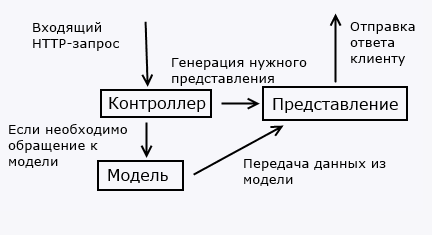
\includegraphics[scale=1.2]{mvc}
	\caption{Паттерн MVC}
	\end{center}
	\end{figure}
	Основная цель применения этой концепции состоит в разделении бизнес-логики (модели) от её визуализации (представления, вида). За счет такого разделения повышается возможность повторного использования. Наиболее полезно применение данной концепции в тех случаях, когда пользователь должен видеть те же самые данные одновременно в различных контекстах и/или с различных точек зрения. В частности, выполняются следующие задачи:\par
	• К одной модели можно присоединить несколько видов, при этом не затрагивая реализацию модели. Например, некоторые данные могут быть одновременно представлены в виде электронной таблицы, гистограммы и круговой диаграммы;\par
	• Не затрагивая реализацию видов, можно изменить реакции на действия пользователя (нажатие мышью на кнопке, ввод данных), для этого достаточно использовать другой контроллер.\par
	Концепция MVC позволяет разделить данные, представление и обработку действий пользователя на три отдельных компонента:\par
	• Модель (англ. Model). Модель предоставляет знания: данные и методы работы с этими данными, реагирует на запросы, изменяя своё состояние. Не содержит информации, как эти знания можно визуализировать;\par
	• Представление, вид (англ. View). Отвечает за отображение информации (визуализацию). Часто в качестве представления выступает форма (окно) с графическими элементами;\par
	• Контроллер (англ. Controller). Обеспечивает связь между пользователем и системой: контролирует ввод данных пользователем и использует модель и представление для реализации необходимой реакции.\par
    	Важно отметить, что как представление, так и контроллер зависят от модели. Однако модель не зависит ни от представления, ни от контроллера.\par

	~\\

	\addcontentsline{toc}{subsection}{1.5 Сервер IIS}
	\textbf{1.5 Сервер IIS}

	\parindent=1cm IIS Web Server встроен в Windows. IIS Express работает с VS 2012 и Visual Web Developer 2010 Express, запускаться на Windows XP и выше, не требует прав администратора и внесения изменений в код приложения. Позволяет работать со всеми типами ASP.NET приложений и разрабатывать, используя всю мощь возможностей IIS 7.x.\par
	Используя IIS, как сервер для разработок получаем все возможности веб-сервера (SSL, URL Rewrite Rules и т.п.). IIS является полноценным веб-сервером, а это значит, что будет точно известно, как будет работать приложения на публичном сервере.\par

	~\\

	\addcontentsline{toc}{subsection}{1.6 Dependency Injection}
	\textbf{1.6 Dependency Injection}

	\parindent=1cm Процесс предоставления внешней зависимости программному компоненту. Является специфичной формой «инверсии управления» (англ. Inversion of control, IoC), где изменение порядка связи осуществляется путём получения необходимой зависимости.\par
	Работа фреймворка, обеспечивающая внедрение зависимости, описывается следующим образом. Приложение, независимо от оформления, исполняется внутри контейнера IoC, предоставляемого фреймворком. Часть объектов в программе по-прежнему создается обычным способом языка программирования, часть создается контейнером на основе предоставленной ему конфигурации.\par
	Условно, если объекту нужно получить доступ к определенному сервису, объект берет на себя ответственность за доступ к этому сервису: он или получает прямую ссылку на местонахождение сервиса, или обращается к известному «сервис-локатору» и запрашивает ссылку на реализацию определенного типа сервиса. Используя же внедрение зависимости, объект просто предоставляет свойство, которое в состоянии хранить ссылку на нужный тип сервиса; и когда объект создается, ссылка на реализацию нужного типа сервиса автоматически вставляется в это свойство (поле), используя средства среды.\par
	Внедрение зависимости более гибко, потому что становится легче создавать альтернативные реализации данного типа сервиса, а потом указывать, какая именно реализация должна быть использована в, например, конфигурационном файле, без изменений в объектах, которые этот сервис используют. Это особенно полезно в юнит-тестировании, потому что вставить реализацию «заглушки» сервиса в тестируемый объект очень просто.\par

	~\\


	%-----СРАВНЕНИЕ АНАЛОГОВ И ПОСТАНОВКА ЗАДАЧИ-----f
	
	\newpage
	\addcontentsline{toc}{section}{2 СРАВНЕНИЕ АНАЛОГОВ И ПОСТАНОВКА ЗАДАЧИ}
	\section*{\normalsize\hspace{4ex}2 СРАВНЕНИЕ АНАЛОГОВ И ПОСТАНОВКА ЗАДАЧИ}
	\addcontentsline{toc}{subsection}{2.1 Сравнение приложения с существующими аналогами}
	\subsection*{\normalsize\hspace{4ex}2.1 Сравнение приложения с существующими аналогами}
	\hspace{2ex} В интернете множество сайтов объявлений, например: kufar.by, ixr.by, doska.by, onliner.by. Данные сайты предусматривают просмотр и поиск объявлений, а также добавление, удаление, изменение объявления. Любой пользователь может зарегистрироваться на сайте и добавить свое объявление(Рис. 2).
	\begin{figure}[h]
	\begin{center}
	\includegraphics[scale=0.45]{kufar_main}
	\caption{Главная страница kufar.by}
	\end{center}
	\end{figure}
	
 	На некоторых сайтах предусмотрена функция отклика на объявления, оставленные другими пользователями(Рис. 3).
	\begin{figure}[h]
	\begin{center}
	\includegraphics[scale=0.45]{kufar_response}
	\caption{Форма отклика на объявление}
	\end{center}
	\end{figure}
		
	 Также у каждого объявления должна быть контактная информация пользователя, разместившего его(Рис. 4).
	\begin{figure}[h]
	\begin{center}
	\includegraphics[scale=0.6]{kufar_contact}
	\caption{Контактная информация владельца объявления}
	\end{center}
	\end{figure}
	
	 На таких сайтах как auto.by необходимо подтверждение администратором объявления . Таким образом администратор осуществляет проверку на цензуру, на сам контент объявления.Это делает сайты приемлимыми и культурными.\par
	Также на многих сайтах объявлений обычно предусмотрена функция редактирования профиля. Пользователи могут указывать свои данные, к примеру: фамилию, имя, телефон, адрес, и тд, если это необходимо. Так клиенту проще связаться с лицом, разместившим объявление.\par
	 На продвинутых сайтах, таких как aliexpress.com можно регистрироваться через сторонние сервисы(Рис. 5). Эта область на данный момент развивается. На многие сайты можно зайти через facebook, vk, google+, yahoo, linkedIn, youtube. Пользователи находят это удобмным и предпочитают аутентифицироваться через сторонние сервисы.\par
	\begin{figure}[h]
	\begin{center}
	\includegraphics[scale=0.45]{ali_auth}
	\caption{Аутентификация через сторонние сервисы}
	\end{center}
	\end{figure}
	
          На данном этапе развития информационных технологий большинство пользователей заинтересовались тэгами. Их можно оставлять везде и всему. Любой сущности можно оставить свой комментарий в виде тэга и не один. Данное приспособление привлекает пользователей, поскольку удобно осуществлять фильтрацию по тэгам. И любой объект можно пометить чем-то своим. Удобно осуществять поиск по тэгам и таким образом сразу находить интересующий нас предмет/область/статью.\par
	 На сайте kufar.by реализован поиск по ключевым словам(Рис. 6). Это обеспечивает технология поиска по ключевым словам сущности, причем не важно, какое это ключевое слово: тэг, название или описание. Так же предусмотрена функция автодополнения, что делает поиск более удобным пользователю.\par
	\begin{figure}[h]
	\begin{center}
	\includegraphics[scale=0.6]{kufar_poisk}
	\caption{Поиск объявлений}
	\end{center}
	\end{figure}
	~\\
	~\\
         Большинтсво сайтов сейчас работают быстро, однако наиболее удобным является технология обновления какой-либо части веб-страницы без ее перезагрузки. К примеру, чтобы "лайк" ставился сразу, чтобы объявление помечалось как "избранное" по щелчку. Поэтому большинство разработчиков стараются предусмотреть такой поворот событий и сделать свое веб-приложение наиболее удобным и комфортным для пользователей(Рис. 7).
	\begin{figure}[h]
	\begin{center}
	\includegraphics[scale=0.6]{kufar_like}
	\caption{Добавление в избранное}
	\end{center}
	\end{figure}
	~\\
	\addcontentsline{toc}{subsection}{2.2 Постановка задачи}
	\subsection*{\normalsize\hspace{4ex}2.2 Постановка задачи}
	\hspace{2ex}Разработать программное средство “Сайт Доска Объявлений” с использованием языка программирования C\#. 


	\hspace{2ex}Реализовать функциональный набор:

	\hspace{2ex}1. Регистрация/вход пользователя в систему;

	\hspace{2ex}2. Просмотр объявлений, размещенных на сайте;

	\hspace{2ex}3. Добавление, изменение, удаление объявлений для зарегистрированных пользователей;

	\hspace{2ex}4. Создание ролей пользователей: администратор и обычный пользователь;

	\hspace{2ex}5. Поиск объявлений;

	\hspace{2ex}6. Добавление изображений для объявлений;\par

          	\hspace{2ex}7. Предусмотреть аутентификацию через сторонние сервисы(vk, google+, facebook),  реализовать возможность редактирования профиля (изменение аутентификационных данных, загрузка аватара), реализовать админку (главный администратор сайта проверяет каждое объявление и разрешает или запрещает его публикацию) \par 
	 Приложение разрабатывать на платформе ASP.NET MVC\par

	%-----РАЗРАБОТКА ПРИЛОЖЕНИЯ----
	\newpage
	\addcontentsline{toc}{section}{3 РАЗРАБОТКА ПРИЛОЖЕНИЯ}
	\section*{\normalsize\hspace{4ex}3 РАЗРАБОТКА ПРИЛОЖЕНИЯ}
	\addcontentsline{toc}{subsection}{3.1 Описание базы данных}
	\subsection*{\normalsize\hspace{4ex}3.1 Описание базы данных}
	\parindent=1cm В данном проекте применялся MS SQL Server для построения базы данных. Доступ к базе осуществляется с помощью Entity Framework (EF) - инфраструктуры ORM для платформы .NET. При помощи Entity Framework таблицы, столбцы и строки реляционной базы данных представляются с помощью обычных объектов C\#. Платформа .NET поддерживает другие инфраструктуры ORM, которые используют разные подходы к орга\-низации и управлению данными, но была выбрана Entity Framework по следующим причинам:\par
	• EF проста и ее легко запустить в работу;\par
	• EF интегрирована с LINQ;\par
	• EF обладает большими функциональными возможностями;\par
	~\\ 
	 Диаграмма IDEF1X базы данных веб-приложения доска объявлений представлена на рисунке 8:
	\begin{figure}[h]
	\begin{center}
	\includegraphics[scale=1]{idef1x}
	\caption{ Диаграмма IDEF1X базы данных}
	\end{center}
	\end{figure}
	~\\
	Основной таблицей является Ad. У отдельного экземляра сущности из таблицы Ad может быть 1 категория объявления, название, описание, дата публикации и уникальный идентификатор пользователя, разместившего объявление.\par
	Структура данных представлена в виде классов.\par

	\addcontentsline{toc}{subsection}{3.2 Используемые классы}
	\subsection*{\normalsize\hspace{4ex}3.2 Используемые классы}
	\parindent=1cmИспользуемые классы:\par
	1)EFAdRepository. Данный класс обеспечивает работу с данными таблиц Ad и Image базы данных. Предоставляет интерфейс для CRUD операций. Содержит поле контекса базы данных (EFDbContext), методы удаления, добавления, сохранения объявлений или картинок. \par
	2)EFDbContext. Класс, устанавливающий связь с таблицами Ad и Image базы данных.\par
	3)Ad, Image. Классы, которые являются объектно-ориентированными представлениями табли Ad и Image базы данных.\par
	4)AccountController. Контроллер, предоставляющий методы регистрации, логина, изменения данных пользователя. Реализуется при помощи Identity 2.0. \par
	5)AdController. Контроллер, предназначенный для работы пользователся с объявлениями (добавление, удаление, просмотр, изменение).\par
	6)AdminController. Контроллер, предназначенный для работы с объявлениями пользователя, обладающего правами администратора.\par
	7)ImageController. Контроллер, в котором содержатся методы загрузки и отображение картинок.\par
	8)UserController. Контроллер, предназначенный для работы пользователя со своими персональными данными и личным кабинетом.\par
	9)NavController. Контроллер, предоставляющий методы для работы с навигационной панелью сайта.\par
	10)IdentityModel. Класс, предоставляющий стандартные модели пользователя в Identity 2.0.\par
	11)UserAdsViewModel. Модель представления, содержащая в себе информацию о конкретном пользователе и все объявления данного пользователя.\par
	12)PagingInfo. Класс, содержащий информацию о пагинации страниц в приложении (общее количество объявлений, максимальное количество объявлений, размещенных на одной странице).\par
	Каждая модель имеет соотвествующий контроллер: AdController, UserController, ImageController\par
	Все роуты происывются в классе RouteConfig, где они заносятся в таблицу роутов, по которой в дальнейшем определяется к какому контроллеру и действию был произведен запрос.\par
	Для организации более эффективной передачи файлов скриптов и стилей, а также для минификации, в классе BundleConfig регистрируются необходимые бандлы.\par
	Что касается представлений, то они написаны с использованием html и движка Razor. Также были разработаны html-хелперы, позволяющие добавлять необходимые html-теги с помощью кода на языке C\#.\par

	%-----ТЕСТИРОВАНИЕ------
	\newpage
	\addcontentsline{toc}{section}{4 ТЕСТИРОВАНИЕ}
	\section*{\normalsize\hspace{4ex}4 ТЕСТИРОВАНИЕ}
	\parindent=1cm Приложение Ad Board покрыто некоторыми тестами. Основная идея юнит тестирования – тестирование отдельных компонентов программы, т.е. классов и их методов. Имеются тесты контроллера, моделей. Для написания тестов использовался Unit Testing Framework NUnit и фреймворк Moq, который позволяют имитировать или эмулировать какую-то функциональность или создавать мок-объекты. \par
	Тесты контроллера включают в себя тестирование:\par
	- AdController;\par
	- UserController;\par
	- AdminController;\par
	Тесты контроллера позволяют протестировать методы контроллера, такие как проверка генерации результата в виде представления, проверка содержимого объявлений и т.д.\par
	Тесты моделей предусматривают тестирование методов класса. В приложении Ad Board была протестирована модель Paging Info.\par
	В приложении были протестированы методы нескольких контроллеров, а также методы моделей. Это свидетельствует о том, что приложение не полностью покрыто тестами, следовательно добавление нового функционала может привести к особым трудностям, поскольку не весь код можно проверить тестами.\par

	%-----РУКОВОДСТВО ПО УСТАНОВКЕ И ИСПОЛЬЗОВАНИЮ ПРИЛОЖЕНИЯ------
	\newpage
	\addcontentsline{toc}{section}{5 РУКОВОДСТВО ПОЛЬЗОВАТЕЛЯ}
	\section*{\normalsize\hspace{4ex}5 РУКОВОДСТВО ПОЛЬЗОВАТЕЛЯ}
	
	\parindent=1cm Так выгляди главная страница сайта.\par
	\begin{figure}[h]
	\begin{center}
	\includegraphics[scale=0.45]{main}
	\caption{Главная страница Ad Board}
	\end{center}
	\end{figure}  

	Для того что бы разместить объявление пользователю необходимо войти на сайт (Рис.10). Для этого он может использовать сторонние сервисы.\par
	\begin{figure}[h]
	\begin{center}
	\includegraphics[scale=0.8]{login}
	\caption{Вход на сайт}
	\end{center}
	\end{figure}  

	Если пользователь хочет зарегестрироваться на сайте он должен заполнить данную форму (Рис. 11).\par
	\begin{figure}[h!]
	\begin{center}
	\includegraphics[scale=0.6]{Register}
	\caption{Регистрация}
	\end{center}
	\end{figure}  
	~\\

	Для изменения своих контактных данных пользователь может воспользоваться редактированием профиля (Рис. 12).\par
	\begin{figure}[h!]
	\begin{center}
	\includegraphics[scale=0.7]{editprofile}
	\caption{Редактирование профиля}
	\end{center}
	\end{figure}  	

	Для того чтобы найти необходимые объявления используется поиск (Рис. 13).\par
	\begin{figure}[h]
	\begin{center}
	\includegraphics[scale=0.8]{poisk}
	\caption{Поиск объявлений}
	\end{center}
	\end{figure}  

	Для просмотра объявлений по нужной категории используется навигационная панель. Соответствующая категория закрашивается, когда данная категория выбрана(Рис. 14).\par
	\begin{figure}[h]
	\begin{center}
	\includegraphics[scale=0.6]{adch}
	\caption{Выбранная категория}
	\end{center}
	\end{figure}  

	Полная информация об объявлении предоставлена на рисунке 15.\par
	\begin{figure}[h!]
	\begin{center}
	\includegraphics[scale=0.7]{adinfo}
	\caption{Информация об объявлении}
	\end{center}
	\end{figure}  
	~\\~\\~\\~\\~\\	~\\~\\~\\~\\~\\

	Просмотр объявлений залогинившегося пользователя предоставлен на рисунке 16.\par
	\begin{figure}[h!]
	\begin{center}
	\includegraphics[scale=0.8]{myads}
	\caption{Мои объявления}
	\end{center}
	\end{figure}  

	Добавление нового оъявления может осуществлять только залогинившийся пользователь. Форма добавления объявления показана на рисунке 17.\par
	\begin{figure}[h]
	\begin{center}
	\includegraphics[scale=0.7]{add}
	\caption{Добавление объявления}
	\end{center}
	\end{figure}  

	Форма редактирования объявления предоставлена на рисунке 18.\par
~\\~\\
	\begin{figure}[h!]
	\begin{center}
	\includegraphics[scale=0.8]{editadd}
	\caption{Редактирование объявления}
	\end{center}
	\end{figure}  

	Также в данном придожении есть панель администратора, которая доступна только тем пользователям, которые наделены соответствующими правами администратора(Рис.19).\par
	\begin{figure}[h]
	\begin{center}
	\includegraphics[scale=0.6]{adminbtn}
	\caption{Панель администратора}
	\end{center}
	\end{figure}  

	Администратор может удалять (Рис. 20) и редактировать объявления (Рис. 21).\par
	\begin{figure}[h]
	\begin{center}
	\includegraphics[scale=0.5]{adminlist}
	\caption{Панель администратора: список объявлений}
	\end{center}
	\end{figure}  

	\begin{figure}[h]
	\begin{center}
	\includegraphics[scale=0.6]{adminedit}
	\caption{Панель администратора: редактирование объявления}
	\end{center}
	\end{figure}  


%-------ЗАКЛЮЧЕНИЕ-------%
	\newpage
	\addcontentsline{toc}{section}{ЗАКЛЮЧЕНИЕ}
	\section*{\center\normalsize ЗАКЛЮЧЕНИЕ \endcenter}


	\parindent=1cm В результате выполнения курсовой работы была изучена возможность регистрации пользователей через Identity. Также были изучены основы реляционных баз данных, в частности MSSql. Были выполнены следующие требования:\par
	- Возможность создания и удаления пользователя;\par
	- Возможность редактирования профиля пользователя (включает загрузку аватара и изменения личных и контактных данных);\par
	- Возможность создания объявления;\par
	- Возможность редактирования и удаления объявления (загрузка фотографий, добавление подробного описания, личных данных человека, разместившего обявление);\par
	- Создание ролей пользователей: админ и простой пользователь. У админа больше полномочий чем у обычного пользователя;\par
	- Технология поиска объявлений ( поиск по названию, категории);\par
	- Предусмотрена аутентификация через сторонние сервисы (vk, google+, facebook);\par
	- Реализовоны дополнительные возможности администраторов сайта (запрещение нецензурных публикаций, просмотр чужих объявлений перед публикацией;\par 

	%----СПИСОК ИСПОЛЬЗОВАННОЙ ЛИТЕРАТУРЫ-------
	\newpage
	\addcontentsline{toc}{section}{СПИСОК ИСПОЛЬЗОВАННОЙ ЛИТЕРАТУРЫ}
	\section*{\center\normalsize СПИСОК ИСПОЛЬЗОВАННОЙ ЛИТЕРАТУРЫ \endcenter}

	\parindent=1cm[1] Википедия [Электронный ресурс]. – Электронные данные. – Режим доступа:						\href{http://ru.wikipedia.org/wiki/}{http://ru.wikipedia.org/wiki/}\par
	[2] Pro Asp.Net MVC - Adam Freeman\par
	[3] CLR via C\# - Jeffrey Richter\par
	[4] Pro C\# 5.0 and the .NET 4.5 Framework - Andrew Troelsen\par

	%----ПРИЛОЖЕНИЕ А (обязательное) Исходный код программы----
	\lstset{style=sharpc}

	\newpage
	\addcontentsline{toc}{section}{ПРИЛОЖЕНИЕ А}
	\section*{\center\normalsize ПРИЛОЖЕНИЕ А\\(обязательное)\\Исходный код программы \endcenter}
	\begin{lstlisting}
using System;
using System.Collections.Generic;
using System.Linq;
using System.Text;
using System.Threading.Tasks;
using System.ComponentModel.DataAnnotations;
using System.Web.Mvc;


namespace AdBoard.Domain.Entities
{
    public class Ad
    {
        [HiddenInput(DisplayValue=false)]
        public int Id { get; set; }
        
        [Required(ErrorMessage="Please, enter ad name")]
        [Display(Name="Name")]
        public string Name { get; set; }

        [DataType(DataType.MultilineText)]
        [Required(ErrorMessage="Please, enter description for ad")]
        public string Description { get; set; }
        
        [DataType(DataType.Date)]
        [DisplayFormat(DataFormatString=("{0:dd/MM/yyyy}"), ApplyFormatInEditMode=true)]
        [Required(ErrorMessage="Please, enter date for ad(use slash\"/\")")]
        public DateTime Date { get; set; }

        [Required(ErrorMessage="Please, enter ad category")]
        [Display(Name="Cateogry")]
        public string Category { get; set; }

        [HiddenInput(DisplayValue=false)]
        public string UserId { get; set; }

        [Required(ErrorMessage = "Please, enter ad price")]
        [DataType(DataType.Currency)]
        public decimal Price { get; set; }

        [HiddenInput(DisplayValue = true)]
        public IEnumerable<Image> Images { get; set; }
    }
}

using System;
using System.Collections.Generic;
using System.Linq;
using System.Text;

namespace AdBoard.Domain.Entities
{
    public class Image
    {
        public int Id { get; set; }
        public int AdId { get; set; }
        public byte[] ImageData { get; set; }
        public string ImageMimeType { get; set; }
    }
}

using AdBoard.Domain.Entities;
using System;
using System.Collections.Generic;
using System.Linq;
using System.Text;
using System.Threading.Tasks;

namespace AdBoard.Domain.Abstract
{
    public interface IAdRepository
    {
        IEnumerable<Ad> Ads { get; }
        IEnumerable<Image> Images { get; }
        void SaveAd(Ad ad);
        Ad DeleteAd(int adId);
        void SaveImage(Image image);
    }
}

using AdBoard.Domain.Entities;
using System;
using System.Collections.Generic;
using System.Data.Entity;
using System.Linq;
using System.Text;
using System.Threading.Tasks;

namespace AdBoard.Domain.Concrete
{
    public class EFDbContext : DbContext
    {
        public DbSet<Ad> Ads { get; set; }
        public DbSet<Image> Images { get; set; }
    }
}

using AdBoard.Domain.Abstract;
using AdBoard.Domain.Entities;
using System;
using System.Collections.Generic;
using System.Linq;
using System.Text;
using System.Threading.Tasks;

namespace AdBoard.Domain.Concrete
{
    public class EFAdRepository : IAdRepository, IDisposable
    {
        EFDbContext context = new EFDbContext();

        public virtual IEnumerable<Entities.Ad> Ads
        {
            get { return context.Ads; }
        }

        public IEnumerable<Entities.Image> Images
        {
            get { return context.Images; }
        }

        public void SaveAd(Ad ad)
        {
            if (ad.Id == 0)
                context.Ads.Add(ad);
            else
            {
                Ad dbEntry = context.Ads.Find(ad.Id);
                if (dbEntry != null)
                {
                    dbEntry.Name = ad.Name;
                    dbEntry.Description = ad.Description;
                    dbEntry.Price = ad.Price;
                    dbEntry.Category = ad.Category;
                    dbEntry.Date = ad.Date;
                }
            }
            context.SaveChanges();
        }
        
        public Ad DeleteAd(int adId)
        {
            Ad dbEntry = context.Ads.Find(adId);
            if (dbEntry != null)
            {
                context.Ads.Remove(dbEntry);
                context.SaveChanges();
            }
            return dbEntry;
        }

        public void SaveImage(Image image)
        {
            if (image.Id == 0)
                context.Images.Add(image);
            else
            {
                Image dbEntry = context.Images.Find(image.Id);
                if (dbEntry != null)
                {
                    dbEntry.AdId = image.AdId;
                    dbEntry.Id = image.Id;
                    dbEntry.ImageData = image.ImageData;
                    dbEntry.ImageMimeType = image.ImageMimeType;
                }
            }
            context.SaveChanges();
        }

        public void Save()
        {
            context.SaveChanges();
        }

        protected void DisposeContext(bool disposing)
        {
            if(disposing)
            {
                if(context != null)
                {
                    context.Dispose();
                    context = null;
                }
            }

        }

        public void Dispose()
        {
            DisposeContext(true);
            GC.SuppressFinalize(this);
        }
    }
}

using System.Web;
using System.Web.Optimization;

namespace AdBoard.WebUI
{
    public class BundleConfig
    {
        // For more information on bundling, visit http://go.microsoft.com/fwlink/?LinkId=301862
        public static void RegisterBundles(BundleCollection bundles)
        {
            bundles.Add(new ScriptBundle("~/bundles/jquery").Include(
                        "~/Scripts/jquery-{version}.js"));

            bundles.Add(new ScriptBundle("~/bundles/jqueryval").Include(
                        "~/Scripts/jquery.validate*"));

            // Use the development version of Modernizr to develop with and learn from. Then, when you're
            // ready for production, use the build tool at http://modernizr.com to pick only the tests you need.
            bundles.Add(new ScriptBundle("~/bundles/modernizr").Include(
                        "~/Scripts/modernizr-*"));

            bundles.Add(new ScriptBundle("~/bundles/bootstrap").Include(
                      "~/Scripts/bootstrap.js",
                      "~/Scripts/respond.js"));

            bundles.Add(new StyleBundle("~/Content/css").Include(
                      "~/Content/bootstrap.css",
                      "~/Content/site.css"));

            bundles.Add(new ScriptBundle("~/bundles/jquerymask").Include(
                        "~/Scripts/jquery.mask.min.js",
                        "~/Scripts/maskedinput-binder.js"));

            bundles.Add(new ScriptBundle("~/bundles/jasny-bootstrap").Include(
                "~/Scripts/jasny-bootstrap.min.js"));

            bundles.Add(new ScriptBundle("~/bundles/imageload").Include(
                "~/Scripts/imageload.js"));

            bundles.Add(new ScriptBundle("~/bundles/sitescripts").Include(
                "~/Scripts/sitescripts.js"));

            // Set EnableOptimizations to false for debugging. For more information,
            // visit http://go.microsoft.com/fwlink/?LinkId=301862
            BundleTable.EnableOptimizations = true;
        }
    }
}

using System.Web;
using System.Web.Mvc;

namespace AdBoard.WebUI
{
    public class FilterConfig
    {
        public static void RegisterGlobalFilters(GlobalFilterCollection filters)
        {
            filters.Add(new HandleErrorAttribute());
        }
    }
}

using System.Threading.Tasks;
using Microsoft.AspNet.Identity;
using Microsoft.AspNet.Identity.EntityFramework;
using Microsoft.AspNet.Identity.Owin;
using Microsoft.Owin;
using AdBoard.WebUI.Models;

namespace AdBoard.WebUI
{
    // Configure the application user manager used in this application. UserManager is defined in ASP.NET Identity and is used by the application.

    public class ApplicationUserManager : UserManager<ApplicationUser>
    {
        public ApplicationUserManager(IUserStore<ApplicationUser> store)
            : base(store)
        {
        }

        public static ApplicationUserManager Create(IdentityFactoryOptions<ApplicationUserManager> options, IOwinContext context) 
        {
            var manager = new ApplicationUserManager(new UserStore<ApplicationUser>(context.Get<ApplicationDbContext>()));
            // Configure validation logic for usernames
            manager.UserValidator = new UserValidator<ApplicationUser>(manager)
            {
                AllowOnlyAlphanumericUserNames = false,
                RequireUniqueEmail = true
            };
            // Configure validation logic for passwords
            manager.PasswordValidator = new PasswordValidator
            {
                RequiredLength = 6,
                RequireNonLetterOrDigit = false,
                RequireDigit = true,
                RequireLowercase = true,
                RequireUppercase = false,
            };
            // Register two factor authentication providers. This application uses Phone and Emails as a step of receiving a code for verifying the user
            // You can write your own provider and plug in here.
            manager.RegisterTwoFactorProvider("PhoneCode", new PhoneNumberTokenProvider<ApplicationUser>
            {
                MessageFormat = "Your security code is: {0}"
            });
            manager.RegisterTwoFactorProvider("EmailCode", new EmailTokenProvider<ApplicationUser>
            {
                Subject = "Security Code",
                BodyFormat = "Your security code is: {0}"
            });
            manager.EmailService = new EmailService();
            manager.SmsService = new SmsService();
            var dataProtectionProvider = options.DataProtectionProvider;
            if (dataProtectionProvider != null)
            {
                manager.UserTokenProvider = new DataProtectorTokenProvider<ApplicationUser>(dataProtectionProvider.Create("ASP.NET Identity"));
            }
            return manager;
        }
    }

    public class EmailService : IIdentityMessageService
    {
        public Task SendAsync(IdentityMessage message)
        {
            // Plug in your email service here to send an email.
            return Task.FromResult(0);
        }
    }

    public class SmsService : IIdentityMessageService
    {
        public Task SendAsync(IdentityMessage message)
        {
            // Plug in your sms service here to send a text message.
            return Task.FromResult(0);
        }
    }
}

[assembly: WebActivatorEx.PreApplicationStartMethod(typeof(AdBoard.WebUI.App_Start.NinjectWebCommon), "Start")]
[assembly: WebActivatorEx.ApplicationShutdownMethodAttribute(typeof(AdBoard.WebUI.App_Start.NinjectWebCommon), "Stop")]

namespace AdBoard.WebUI.App_Start
{
    using System;
    using System.Web;

    using Microsoft.Web.Infrastructure.DynamicModuleHelper;

    using Ninject;
    using Ninject.Web.Common;
    using System.Web.Mvc;
    using AdBoard.WebUI.Infrastructure;

    public static class NinjectWebCommon 
    {
        private static readonly Bootstrapper bootstrapper = new Bootstrapper();

        /// <summary>
        /// Starts the application
        /// </summary>
        public static void Start() 
        {
            DynamicModuleUtility.RegisterModule(typeof(OnePerRequestHttpModule));
            DynamicModuleUtility.RegisterModule(typeof(NinjectHttpModule));
            bootstrapper.Initialize(CreateKernel);
        }
        
        /// <summary>
        /// Stops the application.
        /// </summary>
        public static void Stop()
        {
            bootstrapper.ShutDown();
        }
        
        /// <summary>
        /// Creates the kernel that will manage your application.
        /// </summary>
        /// <returns>The created kernel.</returns>
        private static IKernel CreateKernel()
        {
            var kernel = new StandardKernel();
            try
            {
                kernel.Bind<Func<IKernel>>().ToMethod(ctx => () => new Bootstrapper().Kernel);
                kernel.Bind<IHttpModule>().To<HttpApplicationInitializationHttpModule>();

                RegisterServices(kernel);
                return kernel;
            }
            catch
            {
                kernel.Dispose();
                throw;
            }
        }

        /// <summary>
        /// Load your modules or register your services here!
        /// </summary>
        /// <param name="kernel">The kernel.</param>
        private static void RegisterServices(IKernel kernel)
        {
            DependencyResolver.SetResolver(new NinjectDependencyResolver(kernel));
        }        
    }
}

using System;
using System.Collections.Generic;
using System.Linq;
using System.Web;
using System.Web.Mvc;
using System.Web.Routing;

namespace AdBoard.WebUI
{
    public class RouteConfig
    {
        public static void RegisterRoutes(RouteCollection routes)
        {
            routes.IgnoreRoute("{resource}.axd/{*pathInfo}");

            routes.MapRoute(null,
                "",
                new
                {
                    controller = "Ad",
                    action = "List",
                    category = (string)null,
                    page = 1
                });

            routes.MapRoute(
                null,
                "UserAds{page}",
                new { controller = "User", action = "UserAds" },
                constraints: new { page = @"\d+" }
            );

            routes.MapRoute(
                null,
                "UserAds",
                new { controller = "User", action = "UserAds" }
            );

            routes.MapRoute(
                null,
                "EditProfile",
                new { controller = "Account", action = "EditProfile" }
            );

            routes.MapRoute(
                null,
                "Search",
                new { controller = "Ad", action = "SearchAds" }
            );

            routes.MapRoute(
                name: null,
                url: "AdInfo{id}",
                defaults: new { controller = "Ad", action = "AdInfo" },
                constraints: new { id = @"\d+" }
            );

            routes.MapRoute(
                name: null,
                url: "Page{page}",
                defaults: new { controller = "Ad", action = "List", category = (string)null },
                constraints: new { page = @"\d+"}
            );

            routes.MapRoute(
                null,
                "{category}",
                new { controller = "Ad", action = "List", page = 1}
            );

            routes.MapRoute(
                null,
                "{category}/Page{page}",
                new { controller = "Ad", action = "List"},
                new { page = @"\d+"}
            );

            routes.MapRoute(null, "{controller}/{action}");
        }
    }
}

using Microsoft.AspNet.Identity;
using Microsoft.AspNet.Identity.EntityFramework;
using Microsoft.AspNet.Identity.Owin;
using Microsoft.Owin;
using Microsoft.Owin.Security.Cookies;
using Microsoft.Owin.Security.DataProtection;
using Microsoft.Owin.Security.Google;
using Owin;
using System;
using AdBoard.WebUI.Models;

namespace AdBoard.WebUI
{
    public partial class Startup
    {
        // For more information on configuring authentication, please visit http://go.microsoft.com/fwlink/?LinkId=301864
        public void ConfigureAuth(IAppBuilder app)
        {
            // Configure the db context and user manager to use a single instance per request
            app.CreatePerOwinContext(ApplicationDbContext.Create);
            app.CreatePerOwinContext<ApplicationUserManager>(ApplicationUserManager.Create);

            // Enable the application to use a cookie to store information for the signed in user
            // and to use a cookie to temporarily store information about a user logging in with a third party login provider
            // Configure the sign in cookie
            app.UseCookieAuthentication(new CookieAuthenticationOptions
            {
                AuthenticationType = DefaultAuthenticationTypes.ApplicationCookie,
                LoginPath = new PathString("/Account/Login"),
                Provider = new CookieAuthenticationProvider
                {
                    OnValidateIdentity = SecurityStampValidator.OnValidateIdentity<ApplicationUserManager, ApplicationUser>(
                        validateInterval: TimeSpan.FromMinutes(30),
                        regenerateIdentity: (manager, user) => user.GenerateUserIdentityAsync(manager))
                }
            });
            
            app.UseExternalSignInCookie(DefaultAuthenticationTypes.ExternalCookie);

            // Uncomment the following lines to enable logging in with third party login providers
            //app.UseMicrosoftAccountAuthentication(
            //    clientId: "",
            //    clientSecret: "");

            //app.UseTwitterAuthentication(
            //   consumerKey: "",
            //   consumerSecret: "");

            app.UseFacebookAuthentication(
               appId: "1636839839860813",
               appSecret: "74abcaffe1cede5606bade7524a2cf64");

            app.UseGoogleAuthentication(new GoogleOAuth2AuthenticationOptions()
            {
                ClientId = "1051820490822-b8mo77iknruoecm45kftnncr0l2s2qp1.apps.googleusercontent.com",
                ClientSecret = "dW-HN0Vi-vJFOTmv1pEMiQXQ"
            });

            app.UseVkontakteAuthentication(appId: "4856605", appSecret: "mEtzKiP8KSNKi6hNigJV", scope: "email");
        }
    }
}

using System;
using System.Collections.Generic;
using System.Linq;
using System.Security.Claims;
using System.Threading.Tasks;
using System.Web;
using System.Web.Mvc;
using Microsoft.AspNet.Identity;
using Microsoft.AspNet.Identity.EntityFramework;
using Microsoft.AspNet.Identity.Owin;
using Microsoft.Owin.Security;
using Owin;
using AdBoard.WebUI.Models;

namespace AdBoard.WebUI.Controllers
{
    [Authorize]
    public class AccountController : Controller
    {
        private ApplicationUserManager _userManager;

        public AccountController()
        {
        }

        public AccountController(ApplicationUserManager userManager)
        {
            UserManager = userManager;
        }

        public ApplicationUserManager UserManager {
            get
            {
                return _userManager ?? HttpContext.GetOwinContext().GetUserManager<ApplicationUserManager>();
            }
            private set
            {
                _userManager = value;
            }
        }

        //
        // GET: /Account/Login
        [AllowAnonymous]
        public ActionResult Login(string returnUrl)
        {
            ViewBag.ReturnUrl = returnUrl;
            return View();
        }

        //
        // POST: /Account/Login
        [HttpPost]
        [AllowAnonymous]
        [ValidateAntiForgeryToken]
        public async Task<ActionResult> Login(LoginViewModel model, string returnUrl)
        {
            if (ModelState.IsValid)
            {
                var user = await UserManager.FindAsync(model.Email, model.Password);
                if (user != null)
                {
                    await SignInAsync(user, model.RememberMe);
                    return RedirectToLocal(returnUrl);
                }
                else
                {
                    ModelState.AddModelError("", "Invalid username or password.");
                }
            }

            // If we got this far, something failed, redisplay form
            return View(model);
        }

        //
        // GET: /Account/Register
        [AllowAnonymous]
        public ActionResult Register()
        {
            return View();
        }

        //
        // POST: /Account/Register
        [HttpPost]
        [AllowAnonymous]
        [ValidateAntiForgeryToken]
        public async Task<ActionResult> Register(RegisterViewModel model, HttpPostedFileBase image = null)
        {
            if (ModelState.IsValid)
            {
                var user = new ApplicationUser() { UserName = model.Email, Email = model.Email, Name = model.Name,
                    Surname = model.Surname, Country = model.Country, StreetAddress = model.StreetAddress, 
                    MobilePhone = model.MobilePhone, ImageData = model.ImageData, ImageMimeType = model.ImageMimeType,
                    FavoritesAds = model.FavoritesAds};

                if (image != null)
                {
                    user.ImageMimeType = image.ContentType;
                    user.ImageData = new byte[image.ContentLength];
                    image.InputStream.Read(user.ImageData, 0, image.ContentLength);
                }

                IdentityResult result = await UserManager.CreateAsync(user, model.Password);
                if (result.Succeeded)
                {
                    await UserManager.AddToRoleAsync(user.Id, "user");
                    await SignInAsync(user, isPersistent: false);

                    // For more information on how to enable account confirmation and password reset please visit http://go.microsoft.com/fwlink/?LinkID=320771
                    // Send an email with this link
                    // string code = await UserManager.GenerateEmailConfirmationTokenAsync(user.Id);
                    // var callbackUrl = Url.Action("ConfirmEmail", "Account", new { userId = user.Id, code = code }, protocol: Request.Url.Scheme);
                    // await UserManager.SendEmailAsync(user.Id, "Confirm your account", "Please confirm your account by clicking <a href=\"" + callbackUrl + "\">here</a>");

                    return RedirectToAction("UserAds", "User");
                }
                else
                {
                    AddErrors(result);
                }
            }

            // If we got this far, something failed, redisplay form
            return View(model);
        }

        //
        // GET: /Account/ConfirmEmail
        [AllowAnonymous]
        public async Task<ActionResult> ConfirmEmail(string userId, string code)
        {
            if (userId == null || code == null) 
            {
                return View("Error");
            }

            IdentityResult result = await UserManager.ConfirmEmailAsync(userId, code);
            if (result.Succeeded)
            {
                return View("ConfirmEmail");
            }
            else
            {
                AddErrors(result);
                return View();
            }
        }

        //
        // GET: /Account/ForgotPassword
        [AllowAnonymous]
        public ActionResult ForgotPassword()
        {
            return View();
        }

        //
        // POST: /Account/ForgotPassword
        [HttpPost]
        [AllowAnonymous]
        [ValidateAntiForgeryToken]
        public async Task<ActionResult> ForgotPassword(ForgotPasswordViewModel model)
        {
            if (ModelState.IsValid)
            {
                var user = await UserManager.FindByNameAsync(model.Email);
                if (user == null || !(await UserManager.IsEmailConfirmedAsync(user.Id)))
                {
                    ModelState.AddModelError("", "The user either does not exist or is not confirmed.");
                    return View();
                }

                // For more information on how to enable account confirmation and password reset please visit http://go.microsoft.com/fwlink/?LinkID=320771
                // Send an email with this link
                // string code = await UserManager.GeneratePasswordResetTokenAsync(user.Id);
                // var callbackUrl = Url.Action("ResetPassword", "Account", new { userId = user.Id, code = code }, protocol: Request.Url.Scheme);		
                // await UserManager.SendEmailAsync(user.Id, "Reset Password", "Please reset your password by clicking <a href=\"" + callbackUrl + "\">here</a>");
                // return RedirectToAction("ForgotPasswordConfirmation", "Account");
            }

            // If we got this far, something failed, redisplay form
            return View(model);
        }

        //
        // GET: /Account/ForgotPasswordConfirmation
        [AllowAnonymous]
        public ActionResult ForgotPasswordConfirmation()
        {
            return View();
        }
	
        //
        // GET: /Account/ResetPassword
        [AllowAnonymous]
        public ActionResult ResetPassword(string code)
        {
            if (code == null) 
            {
                return View("Error");
            }
            return View();
        }

        //
        // POST: /Account/ResetPassword
        [HttpPost]
        [AllowAnonymous]
        [ValidateAntiForgeryToken]
        public async Task<ActionResult> ResetPassword(ResetPasswordViewModel model)
        {
            if (ModelState.IsValid)
            {
                var user = await UserManager.FindByNameAsync(model.Email);
                if (user == null)
                {
                    ModelState.AddModelError("", "No user found.");
                    return View();
                }
                IdentityResult result = await UserManager.ResetPasswordAsync(user.Id, model.Code, model.Password);
                if (result.Succeeded)
                {
                    return RedirectToAction("ResetPasswordConfirmation", "Account");
                }
                else
                {
                    AddErrors(result);
                    return View();
                }
            }

            // If we got this far, something failed, redisplay form
            return View(model);
        }

        //
        // GET: /Account/ResetPasswordConfirmation
        [AllowAnonymous]
        public ActionResult ResetPasswordConfirmation()
        {
            return View();
        }

        //
        // POST: /Account/Disassociate
        [HttpPost]
        [ValidateAntiForgeryToken]
        public async Task<ActionResult> Disassociate(string loginProvider, string providerKey)
        {
            ManageMessageId? message = null;
            IdentityResult result = await UserManager.RemoveLoginAsync(User.Identity.GetUserId(), new UserLoginInfo(loginProvider, providerKey));
            if (result.Succeeded)
            {
                var user = await UserManager.FindByIdAsync(User.Identity.GetUserId());
                await SignInAsync(user, isPersistent: false);
                message = ManageMessageId.RemoveLoginSuccess;
            }
            else
            {
                message = ManageMessageId.Error;
            }
            return RedirectToAction("Manage", new { Message = message });
        }

        //
        // GET: /Account/Manage
        public ActionResult Manage(ManageMessageId? message)
        {
            ViewBag.StatusMessage =
                message == ManageMessageId.ChangePasswordSuccess ? "Your password has been changed."
                : message == ManageMessageId.SetPasswordSuccess ? "Your password has been set."
                : message == ManageMessageId.RemoveLoginSuccess ? "The external login was removed."
                : message == ManageMessageId.Error ? "An error has occurred."
                : "";
            ViewBag.HasLocalPassword = HasPassword();
            ViewBag.ReturnUrl = Url.Action("Manage");
            return View();
        }

        //
        // POST: /Account/Manage
        [HttpPost]
        [ValidateAntiForgeryToken]
        public async Task<ActionResult> Manage(ManageUserViewModel model)
        {
            bool hasPassword = HasPassword();
            ViewBag.HasLocalPassword = hasPassword;
            ViewBag.ReturnUrl = Url.Action("Manage");
            if (hasPassword)
            {
                if (ModelState.IsValid)
                {
                    IdentityResult result = await UserManager.ChangePasswordAsync(User.Identity.GetUserId(), model.OldPassword, model.NewPassword);
                    if (result.Succeeded)
                    {
                        var user = await UserManager.FindByIdAsync(User.Identity.GetUserId());
                        await SignInAsync(user, isPersistent: false);
                        return RedirectToAction("Manage", new { Message = ManageMessageId.ChangePasswordSuccess });
                    }
                    else
                    {
                        AddErrors(result);
                    }
                }
            }
            else
            {
                // User does not have a password so remove any validation errors caused by a missing OldPassword field
                ModelState state = ModelState["OldPassword"];
                if (state != null)
                {
                    state.Errors.Clear();
                }

                if (ModelState.IsValid)
                {
                    IdentityResult result = await UserManager.AddPasswordAsync(User.Identity.GetUserId(), model.NewPassword);
                    if (result.Succeeded)
                    {
                        return RedirectToAction("Manage", new { Message = ManageMessageId.SetPasswordSuccess });
                    }
                    else
                    {
                        AddErrors(result);
                    }
                }
            }

            // If we got this far, something failed, redisplay form
            return View(model);
        }

        public ActionResult EditProfile()
        {
            ManageUserViewModel model = new ManageUserViewModel();
            var user = UserManager.FindById(User.Identity.GetUserId());

            model.Name = user.Name;
            model.Surname = user.Surname;
            model.MobilePhone = user.MobilePhone;
            model.Email = user.Email;
            model.Country = user.Country;
            model.StreetAddress = user.StreetAddress;
            model.OldPassword = string.Empty;
            model.NewPassword = string.Empty;
            return View(model);
        }

        [HttpPost]
        [ValidateAntiForgeryToken]
        public async Task<ActionResult> EditProfile(ManageUserViewModel model, HttpPostedFileBase image = null)
        {
            if (ModelState.IsValid)
            {
                var user = UserManager.FindById(User.Identity.GetUserId());

                user.Name = model.Name;
                user.Surname = model.Surname;
                user.MobilePhone = model.MobilePhone;
                user.Email = model.Email;
                user.Country = model.Country;
                user.StreetAddress = model.StreetAddress;
                if (image != null)
                {
                    user.ImageMimeType = image.ContentType;
                    user.ImageData = new byte[image.ContentLength];
                    image.InputStream.Read(user.ImageData, 0, image.ContentLength);
                }

                var result = await UserManager.UpdateAsync(user);

                if (!result.Succeeded)
                {
                    AddErrors(result);
                }
            }

            return RedirectToAction("EditProfile");
        }

        //
        // POST: /Account/ExternalLogin
        [HttpPost]
        [AllowAnonymous]
        [ValidateAntiForgeryToken]
        public ActionResult ExternalLogin(string provider, string returnUrl)
        {
            // Request a redirect to the external login provider
            return new ChallengeResult(provider, Url.Action("ExternalLoginCallback", "Account", new { ReturnUrl = returnUrl }));
        }

        //
        // GET: /Account/ExternalLoginCallback
        [AllowAnonymous]
        public async Task<ActionResult> ExternalLoginCallback(string returnUrl)
        {
            var loginInfo = await AuthenticationManager.GetExternalLoginInfoAsync();
            if (loginInfo == null)
            {
                return RedirectToAction("Login");
            }

            // Sign in the user with this external login provider if the user already has a login
            var user = await UserManager.FindAsync(loginInfo.Login);
            if (user != null)
            {
                user.Country = String.Empty;
                user.MobilePhone = String.Empty;
                user.Name = String.Empty;
                user.Surname = String.Empty;
                user.StreetAddress = String.Empty;
                await SignInAsync(user, isPersistent: false);
                return RedirectToLocal(returnUrl);
            }
            else
            {
                // If the user does not have an account, then prompt the user to create an account
                ViewBag.ReturnUrl = returnUrl;
                ViewBag.LoginProvider = loginInfo.Login.LoginProvider;
                return View("ExternalLoginConfirmation", new ExternalLoginConfirmationViewModel { Email = loginInfo.Email });
            }
        }

        //
        // POST: /Account/LinkLogin
        [HttpPost]
        [ValidateAntiForgeryToken]
        public ActionResult LinkLogin(string provider)
        {
            // Request a redirect to the external login provider to link a login for the current user
            return new ChallengeResult(provider, Url.Action("LinkLoginCallback", "Account"), User.Identity.GetUserId());
        }

        //
        // GET: /Account/LinkLoginCallback
        public async Task<ActionResult> LinkLoginCallback()
        {
            var loginInfo = await AuthenticationManager.GetExternalLoginInfoAsync(XsrfKey, User.Identity.GetUserId());
            if (loginInfo == null)
            {
                return RedirectToAction("Manage", new { Message = ManageMessageId.Error });
            }
            IdentityResult result = await UserManager.AddLoginAsync(User.Identity.GetUserId(), loginInfo.Login);
            if (result.Succeeded)
            {
                return RedirectToAction("Manage");
            }
            return RedirectToAction("Manage", new { Message = ManageMessageId.Error });
        }

        //
        // POST: /Account/ExternalLoginConfirmation
        [HttpPost]
        [AllowAnonymous]
        [ValidateAntiForgeryToken]
        public async Task<ActionResult> ExternalLoginConfirmation(ExternalLoginConfirmationViewModel model, string returnUrl)
        {
            if (User.Identity.IsAuthenticated)
            {
                return RedirectToAction("Manage");
            }

            if (ModelState.IsValid)
            {
                // Get the information about the user from the external login provider
                var info = await AuthenticationManager.GetExternalLoginInfoAsync();
                if (info == null)
                {
                    return View("ExternalLoginFailure");
                }
                var user = new ApplicationUser() { UserName = model.Email, Email = model.Email };
                IdentityResult result = await UserManager.CreateAsync(user);
                if (result.Succeeded)
                {
                    result = await UserManager.AddLoginAsync(user.Id, info.Login);
                    if (result.Succeeded)
                    {
                        await SignInAsync(user, isPersistent: false);
                        
                        // For more information on how to enable account confirmation and password reset please visit http://go.microsoft.com/fwlink/?LinkID=320771
                        // Send an email with this link
                        // string code = await UserManager.GenerateEmailConfirmationTokenAsync(user.Id);
                        // var callbackUrl = Url.Action("ConfirmEmail", "Account", new { userId = user.Id, code = code }, protocol: Request.Url.Scheme);
                        // SendEmail(user.Email, callbackUrl, "Confirm your account", "Please confirm your account by clicking this link");
                        
                        return RedirectToLocal(returnUrl);
                    }
                }
                AddErrors(result);
            }

            ViewBag.ReturnUrl = returnUrl;
            return View(model);
        }

        //
        // POST: /Account/LogOff
        [HttpPost]
        [ValidateAntiForgeryToken]
        public ActionResult LogOff()
        {
            AuthenticationManager.SignOut();
            return RedirectToAction("List", "Ad");
        }

        //
        // GET: /Account/ExternalLoginFailure
        [AllowAnonymous]
        public ActionResult ExternalLoginFailure()
        {
            return View();
        }

        [ChildActionOnly]
        public ActionResult RemoveAccountList()
        {
            var linkedAccounts = UserManager.GetLogins(User.Identity.GetUserId());
            ViewBag.ShowRemoveButton = HasPassword() || linkedAccounts.Count > 1;
            return (ActionResult)PartialView("_RemoveAccountPartial", linkedAccounts);
        }

        protected override void Dispose(bool disposing)
        {
            if (disposing && UserManager != null)
            {
                UserManager.Dispose();
                UserManager = null;
            }
            base.Dispose(disposing);
        }

        #region Helpers
        // Used for XSRF protection when adding external logins
        private const string XsrfKey = "XsrfId";

        private IAuthenticationManager AuthenticationManager
        {
            get
            {
                return HttpContext.GetOwinContext().Authentication;
            }
        }

        private async Task SignInAsync(ApplicationUser user, bool isPersistent)
        {
            AuthenticationManager.SignOut(DefaultAuthenticationTypes.ExternalCookie);
            AuthenticationManager.SignIn(new AuthenticationProperties() { IsPersistent = isPersistent }, await user.GenerateUserIdentityAsync(UserManager));
        }

        private void AddErrors(IdentityResult result)
        {
            foreach (var error in result.Errors)
            {
                ModelState.AddModelError("", error);
            }
        }

        private bool HasPassword()
        {
            var user = UserManager.FindById(User.Identity.GetUserId());
            if (user != null)
            {
                return user.PasswordHash != null;
            }
            return false;
        }

        private void SendEmail(string email, string callbackUrl, string subject, string message)
        {
            // For information on sending mail, please visit http://go.microsoft.com/fwlink/?LinkID=320771
        }

        public enum ManageMessageId
        {
            ChangePasswordSuccess,
            SetPasswordSuccess,
            RemoveLoginSuccess,
            Error
        }

        private ActionResult RedirectToLocal(string returnUrl)
        {
            if (Url.IsLocalUrl(returnUrl))
            {
                return Redirect(returnUrl);
            }
            else
            {
                return RedirectToAction("UserAds","User");
            }
        }

        private class ChallengeResult : HttpUnauthorizedResult
        {
            public ChallengeResult(string provider, string redirectUri) : this(provider, redirectUri, null)
            {
            }

            public ChallengeResult(string provider, string redirectUri, string userId)
            {
                LoginProvider = provider;
                RedirectUri = redirectUri;
                UserId = userId;
            }

            public string LoginProvider { get; set; }
            public string RedirectUri { get; set; }
            public string UserId { get; set; }

            public override void ExecuteResult(ControllerContext context)
            {
                var properties = new AuthenticationProperties() { RedirectUri = RedirectUri };
                if (UserId != null)
                {
                    properties.Dictionary[XsrfKey] = UserId;
                }
                context.HttpContext.GetOwinContext().Authentication.Challenge(properties, LoginProvider);
            }
        }
        #endregion

    }
}

using AdBoard.Domain.Abstract;
using AdBoard.Domain.Concrete;
using AdBoard.Domain.Entities;
using AdBoard.WebUI.Models;
using System;
using System.Collections.Generic;
using System.IO;
using System.Linq;
using System.Web;
using System.Web.Mvc;
using Microsoft.AspNet.Identity;


namespace AdBoard.WebUI.Controllers
{
    public class AdController : Controller
    {
        IAdRepository repository;
        public int pageSize = 2;
        protected ApplicationDbContext ApplicationDbContext { get; set; }
        
        public AdController(IAdRepository repo)
        {
            this.ApplicationDbContext = new ApplicationDbContext();
            repository = repo;
        }

        public ViewResult Edit(int id)
        {
            Ad ad = repository.Ads
                    .FirstOrDefault(a => a.Id == id);
            return View(ad);
        }

        [HttpPost]
        public ActionResult Edit(Ad ad)
        {
            if (ModelState.IsValid)
            {
                repository.SaveAd(ad);
                TempData["message"] = string.Format("Changing in ad \"{0}\" was saved", ad.Name);
                return RedirectToAction("UserAds","User");
            }
            else
            {
                return View(ad);
            }
        }

        [HttpPost]
        public ActionResult Delete(int adId)
        {
            Ad deletedAd = repository.DeleteAd(adId);
            if (deletedAd != null)
            {
                TempData["message"] = string.Format("Ad \"{0}\" was deleted",
                    deletedAd.Name);
            }
            return RedirectToAction("UserAds","User");
        }

        public ViewResult Create()
        {
            Ad ad = new Ad();
            ad.UserId = User.Identity.GetUserId();
            return View("Edit", ad);
        }

        public ViewResult List(string category, int page = 1)
        {
            AdListViewModel model = new AdListViewModel
            {
                Ads = repository.Ads
                    .Where(p => category == null || p.Category == category)
                    .OrderBy(ads => ads.Id)
                    .Skip((page - 1) * pageSize)
                    .Take(pageSize).ToList(),
                PagingInfo = new PagingInfo
                {
                    CurrentPage = page,
                    ItemsPerPage = pageSize,
                    TotalItems = category == null ?
                    repository.Ads.Count() :
                    repository.Ads.Where(a => a.Category == category).Count(),
                },
                CurrentCategory = category
            };
            foreach(Ad ad in model.Ads)
            {
                ad.Images = repository.Images
                            .Where(i => i.AdId == ad.Id);       
            }
            ViewBag.IsInfo = false;
            ViewBag.IsUserAd = false;
            return View(model);
        }

        public ViewResult AdInfo(int id)
        {
            var ad = repository.Ads.Where(a => a.Id == id).FirstOrDefault();
            ad.Images = repository.Images.Where(m => m.AdId == id);
            UserAdViewModel model = new UserAdViewModel
            {
                Ad = ad,
                User = ApplicationDbContext.Users.FirstOrDefault(u => u.Id == ad.UserId)
            };
            ViewBag.IsInfo = true;
            ViewBag.IsUserAd = false;
            if (User.Identity.IsAuthenticated)
            {
                if (model.Ad.UserId == User.Identity.GetUserId())
                    ViewBag.IsUserAd = true;
                else
                    ViewBag.IsUserAd = false;
            }
            return View(model);
        }        

        public ActionResult SearchAds(string adName, string category)
        {
            ViewBag.Category = new SelectList(repository.Ads, "Category", "Category");
            ViewBag.IsInfo = false;
            ViewBag.IsUserAd = false;
            var ads = from a in repository.Ads
                      select a;
            if (!String.IsNullOrEmpty(adName))
            {
                ads = ads.Where(a => a.Name.ToLower().Contains(adName.ToLower()));
            }
            if (!String.IsNullOrEmpty(category))
            {
                return View(ads.Where(x => x.Category == category));
            }
            else
                return View(ads);
        }

        public FileContentResult GetAdImage(int imageId)
        {
            var Image = repository.Images.Where(i => i.Id == imageId).FirstOrDefault();
            if (Image != null)
            {
                return File(Image.ImageData, Image.ImageMimeType);
            }
            else
            {
                return null;
                /*string path = AppDomain.CurrentDomain.BaseDirectory + "/Content/Images/No_image.png";
                return File(System.IO.File.ReadAllBytes(path), "image/jpg");*/
            }
        }

        public ActionResult EditImages(int adId)
        {
            var images = repository.Images.Where(i => i.AdId == adId);
            ViewBag.AdId = adId;
            return View(images);
        }

        [HttpPost]
        [ValidateAntiForgeryToken]
        public ActionResult EditImages(int adId, HttpPostedFileBase file = null)
        {
            Image image = new Image();
            if (ModelState.IsValid)
            {
                if (file != null)
                {
                    image.AdId = adId;
                    image.ImageMimeType = file.ContentType;
                    image.ImageData = new byte[file.ContentLength];
                    file.InputStream.Read(image.ImageData, 0, file.ContentLength);

                    repository.SaveImage(image);
                }
               
            }
            else
            {
                return null;                
            }
            return RedirectToAction("AdInfo", new { id = image.AdId });
        }
    }
}

using AdBoard.Domain.Abstract;
using AdBoard.Domain.Entities;
using System;
using System.Collections.Generic;
using System.Linq;
using System.Web;
using System.Web.Mvc;

namespace AdBoard.WebUI.Controllers
{
    public class AdminController : Controller
    {
        IAdRepository repository;

        public AdminController(IAdRepository repo)
        {
            repository = repo;
        }

        public ViewResult Index()
        {
            return View(repository.Ads);
        }

        public ViewResult Edit(int adId)
        {
            Ad ad = repository.Ads.FirstOrDefault(a => a.Id == adId);
            return View(ad);
        }

        [HttpPost]
        public ActionResult Edit(Ad ad)
        {
            if (ModelState.IsValid)
            {
                repository.SaveAd(ad);
                TempData["message"] = string.Format("Changes in ad {0} was saved",
                                                    ad.Name);
                return RedirectToAction("Index");
            }
            else
            {
                return View(ad);
            }
        }

        [HttpPost]
        public ActionResult Delete(int adId)
        {
            Ad deletedAd = repository.DeleteAd(adId);
            if (deletedAd != null)
            {
                TempData["message"] = string.Format("Ad {0} was deleted",
                    deletedAd.Name);
            }
            return RedirectToAction("Index");
        }
    }
}

using AdBoard.WebUI.Models;
using System;
using System.Collections.Generic;
using System.Linq;
using System.Web;
using System.Web.Mvc;

namespace AdBoard.WebUI.Controllers
{
    public class ImageController : Controller
    {
        private ApplicationDbContext contextIdentity = new ApplicationDbContext();

        public ImageController()
        {

        }

        public FileContentResult GetImage(string id)
        {
            ApplicationUser user = contextIdentity.Users.FirstOrDefault(u => u.Id == id);
            if (user != null)
            {
                if (user.ImageData != null)
                    return File(user.ImageData, user.ImageMimeType);
                else
                {
                    string path = AppDomain.CurrentDomain.BaseDirectory + "/Content/Images/User.png";
                    return File(System.IO.File.ReadAllBytes(path), "image/jpg");
                }
            }
            else
                return null;
        }

        protected override void Dispose(bool disposing)
        {
            contextIdentity.Dispose();
            base.Dispose(disposing);
        }
    }
}

using AdBoard.Domain.Abstract;
using AdBoard.Domain.Concrete;
using System;
using System.Collections.Generic;
using System.Linq;
using System.Web;
using System.Web.Mvc;

namespace AdBoard.WebUI.Controllers
{
    public class NavController : Controller
    {
        private IAdRepository repository;

        public NavController(IAdRepository repo)
        {
            repository = repo;
        }

        public PartialViewResult Menu(string category = null)
        {
            ViewBag.SelectedCategory = category;

            IEnumerable<string> categories = repository.Ads
                .Select(a => a.Category)
                .Distinct()
                .OrderBy(x => x);

            return PartialView("FlexMenu", categories);
        }
    }
}

using AdBoard.Domain.Abstract;
using AdBoard.Domain.Entities;
using AdBoard.WebUI.Models;
using System;
using System.Collections.Generic;
using System.Linq;
using System.Web;
using System.Web.Mvc;
using System.Web.Security;
using Microsoft.AspNet.Identity;
using Microsoft.AspNet.Identity.EntityFramework;
using AdBoard.Domain.Concrete;

namespace AdBoard.WebUI.Controllers
{
    public class UserController : Controller
    {
        IAdRepository repository;
        public int pageSize = 1;
        protected ApplicationDbContext ApplicationDbContext { get; set; }

        public UserController(IAdRepository repo)
        {
            this.ApplicationDbContext = new ApplicationDbContext();
            repository = repo;
        }

        public ActionResult UserAds(int page = 1)
        {
            var userId = User.Identity.GetUserId();

            UserAdsViewModel model = new UserAdsViewModel
            {
                Ads = repository.Ads
                    .Where(a => a.UserId == userId)
                    .OrderBy(a => a.Name)
                    .Skip((page - 1) * pageSize)
                    .Take(pageSize)
                    .ToList(),
                PagingInfo = new PagingInfo
                {
                    CurrentPage = page,
                    ItemsPerPage = pageSize,
                    TotalItems = repository.Ads
                        .Where(a => a.UserId == userId)
                        .Count()
                },
                User = ApplicationDbContext.Users.FirstOrDefault(x => x.Id == userId)
            };
            foreach (Ad ad in model.Ads)
            {
                ad.Images = repository.Images
                            .Where(i => i.AdId == ad.Id);
            }
            ViewBag.IsInfo = true;
            ViewBag.IsUserAd = true;
            return View(model);
        }

        public PartialViewResult Profile()
        {
            var userId = User.Identity.GetUserId();
            var user = ApplicationDbContext.Users.FirstOrDefault(x => x.Id == userId);
            return PartialView(user);
        }
    }
}

using System.ComponentModel.DataAnnotations;

namespace AdBoard.WebUI.Models
{
    public class ExternalLoginConfirmationViewModel
    {
        [Required]
        [EmailAddress]
        [Display(Name = "Email")]
        public string Email { get; set; }
    }

    public class ExternalLoginListViewModel
    {
        public string Action { get; set; }
        public string ReturnUrl { get; set; }
    }

    public class ManageUserViewModel
    {
        [Required]
        [EmailAddress]
        [Display(Name="Email")]
        public string Email { get; set; }

        [Required]
        [Display(Name = "Name")]
        public string Name { get; set; }

        [Required]
        [Display(Name = "Surname")]
        public string Surname { get; set; }

        [Required]
        [Display(Name = "Country")]
        public string Country { get; set; }

        [Required]
        [Display(Name = "Street Address")]
        public string StreetAddress { get; set; }

        [Required]
        [Display(Name = "MobilePhone")]
        public string MobilePhone { get; set; }

        [Required]
        [DataType(DataType.Password)]
        [Display(Name = "Current password")]
        public string OldPassword { get; set; }

        [Required]
        [StringLength(100, ErrorMessage = "The {0} must be at least {2} characters long.", MinimumLength = 6)]
        [DataType(DataType.Password)]
        [Display(Name = "New password")]
        public string NewPassword { get; set; }

        [DataType(DataType.Password)]
        [Display(Name = "Confirm new password")]
        [Compare("NewPassword", ErrorMessage = "The new password and confirmation password do not match.")]
        public string ConfirmPassword { get; set; }
    }

    public class LoginViewModel
    {
        [Required]
        [EmailAddress]
        [Display(Name = "Email")]
        public string Email { get; set; }

        [Required]
        [DataType(DataType.Password)]
        [Display(Name = "Password")]
        public string Password { get; set; }

        [Display(Name = "Remember me?")]
        public bool RememberMe { get; set; }
    }

    public class RegisterViewModel
    {
        [Required]
        [EmailAddress]
        [Display(Name = "Email*")]
        public string Email { get; set; }
        
        [Required]
        [Display(Name = "Name*")]
        public string Name { get; set; }
        
        [Required]
        [Display(Name = "Surname*")]
        public string Surname { get; set; }

        [Required]
        [Display(Name = "Country*")]
        public string Country { get; set; }

        [Required]
        [Display(Name="Street Address*")]
        public string StreetAddress { get; set; }

        [Required]
        [Display(Name = "MobilePhone*")]
        public string MobilePhone { get; set; }

        public int[] FavoritesAds { get; set; }

        [Display(Name = "Image")]
        public byte[] ImageData { get; set; }

        public string ImageMimeType { get; set; }


        [Required]
        [StringLength(100, ErrorMessage = "The {0} must be at least {2} characters long.", MinimumLength = 6)]
        [DataType(DataType.Password)]
        [Display(Name = "Password*")]
        public string Password { get; set; }

        [DataType(DataType.Password)]
        [Display(Name = "Confirm password*")]
        [Compare("Password", ErrorMessage = "The password and confirmation password do not match.")]
        public string ConfirmPassword { get; set; }
    }

    public class ResetPasswordViewModel
    {
        [Required]
        [EmailAddress]
        [Display(Name = "Email")]
        public string Email { get; set; }

        [Required]
        [StringLength(100, ErrorMessage = "The {0} must be at least {2} characters long.", MinimumLength = 6)]
        [DataType(DataType.Password)]
        [Display(Name = "Password")]
        public string Password { get; set; }

        [DataType(DataType.Password)]
        [Display(Name = "Confirm password")]
        [Compare("Password", ErrorMessage = "The password and confirmation password do not match.")]
        public string ConfirmPassword { get; set; }

        public string Code { get; set; }
    }

    public class ForgotPasswordViewModel
    {
        [Required]
        [EmailAddress]
        [Display(Name = "Email")]
        public string Email { get; set; }
    }
}

using System;
using System.Collections.Generic;
using System.Linq;
using System.Web;

namespace AdBoard.WebUI.Models
{
    public class PagingInfo
    {
        public int TotalItems { get; set; }
        public int ItemsPerPage { get; set; }
        public int CurrentPage { get; set; }
        public int TotalPages
        {
            get { return (int)Math.Ceiling((decimal)TotalItems / ItemsPerPage); }
        }
    }
}

\end{lstlisting}
	%----ПРИЛОЖЕНИЕ Б (обязательное) Исходный код программы----
	\lstset{style=sharpc}

	\newpage
	\addcontentsline{toc}{section}{ПРИЛОЖЕНИЕ Б}
	\section*{\center\normalsize ПРИЛОЖЕНИЕ Б Исходный код тестов \endcenter}
	\begin{lstlisting}
	using System;
using Microsoft.VisualStudio.TestTools.UnitTesting;
using Moq;
using AdBoard.Domain.Abstract;
using AdBoard.Domain.Entities;
using System.Collections.Generic;
using AdBoard.WebUI.Controllers;
using System.Linq;
using System.Web.Mvc;
using AdBoard.WebUI.Models;
using AdBoard.WebUI.HtmlHelpers;
using Microsoft.AspNet.Identity;
using AdBoard.Domain.Concrete;
using System.Security.Principal;
using System.Threading;
using System.Web;
using System.Web.Routing;
using System.Security.Claims;

namespace AdBoard.UnitTests
{
    [TestClass]
    public class UnitTest1
    {
        [TestMethod]
        public void CanPaginate()
        {
            //arrange
            Mock<IAdRepository> mock = new Mock<IAdRepository>();
            mock.Setup(m => m.Ads).Returns(new List<Ad>
                {
                    new Ad { Id = 1, Name = "A1"},
                    new Ad { Id = 2, Name = "A2"},
                    new Ad { Id = 3, Name = "A3"},
                    new Ad { Id = 4, Name = "A4"},
                    new Ad { Id = 5, Name = "A5"}
                });
            AdController controller = new AdController(mock.Object);
            controller.pageSize = 3;

            //act
            AdListViewModel result = (AdListViewModel)controller.List(null,2).Model;

            //assert
            List<Ad> ads = result.Ads.ToList();
            Assert.IsTrue(ads.Count == 2);
            Assert.AreEqual(ads[0].Name, "A4");
            Assert.AreEqual(ads[1].Name, "A5");
        }

        [TestMethod]
        public void Can_Generate_Page_Links()
        {
            //arrange
            HtmlHelper helper = null;

            PagingInfo pagingInfo = new PagingInfo
            {
                CurrentPage = 2,
                ItemsPerPage = 10,
                TotalItems = 28
            };

            Func<int, string> pageUrlDelegate = i => "Page" + i;

            //act
            MvcHtmlString result = helper.PageLinks(pagingInfo, pageUrlDelegate);

            //asset
            Assert.AreEqual(result.ToString() ,@"<a class=""btn btn-default"" href=""Page1"">1</a>"
                + @"<a class=""btn btn-default btn-primary selected"" href=""Page2"">2</a>"
                + @"<a class=""btn btn-default"" href=""Page3"">3</a>");
        }

        [TestMethod]
        public void Can_Send_Pagination_View_Model()
        {
            //arrange
            Mock<IAdRepository> mock = new Mock<IAdRepository>();
            mock.Setup(m => m.Ads).Returns(new List<Ad>
            {
                new Ad { Id = 1, Name = "A1"},
                    new Ad { Id = 2, Name = "A2"},
                    new Ad { Id = 3, Name = "A3"},
                    new Ad { Id = 4, Name = "A4"},
                    new Ad { Id = 5, Name = "A5"}
            });
            AdController controller = new AdController(mock.Object);
            controller.pageSize = 3;

            //act
            AdListViewModel result = (AdListViewModel)controller.List(null,2).Model;

            //assert
            PagingInfo pagingInfo = result.PagingInfo;
            Assert.AreEqual(pagingInfo.CurrentPage, 2);
            Assert.AreEqual(pagingInfo.TotalItems, 5);
            Assert.AreEqual(pagingInfo.TotalPages, 2);
            Assert.AreEqual(pagingInfo.ItemsPerPage, 3);
        }

        [TestMethod]
        public void Can_Filter_Ads()
        {
            //arrange
            Mock<IAdRepository> mock = new Mock<IAdRepository>();
            mock.Setup(m => m.Ads).Returns(new List<Ad>
            {
                new Ad { Id = 1, Name = "Ad1", Category = "C1"},
                new Ad { Id = 2, Name = "Ad2", Category = "C2"},
                new Ad { Id = 3, Name = "Ad3", Category = "C1"},
                new Ad { Id = 4, Name = "Ad4", Category = "C2"},
                new Ad { Id = 5, Name = "Ad5", Category = "C1"}
            });
            AdController controller = new AdController(mock.Object);
            controller.pageSize = 3;

            //act
            List<Ad> result = ((AdListViewModel)controller.List("C2", 1).Model).Ads.ToList();

            //assert
            Assert.AreEqual(result.Count, 2);
            Assert.IsTrue(result[0].Name == "Ad2" && result[0].Category == "C2");
            Assert.IsTrue(result[1].Name == "Ad4" && result[1].Category == "C2");
        }

        [TestMethod]
        public void Can_Generate_List_of_Categories()
        {
            Mock<IAdRepository> mock = new Mock<IAdRepository>();
            mock.Setup(m => m.Ads).Returns(new List<Ad>
                {
                    new Ad { Id = 1, Category = "C1"},
                    new Ad { Id = 2, Category = "C3"},
                    new Ad { Id = 3, Category = "C1"},
                    new Ad { Id = 4, Category = "C2"},
                    new Ad { Id = 5, Category = "C3"},
                });
            NavController controller = new NavController(mock.Object);

            //act
            List<string> result = ((IEnumerable<string>)controller.Menu(null).Model).ToList();

            //assert
            Assert.IsTrue(result.Count == 3);
            Assert.AreEqual(result[0], "C1");
            Assert.AreEqual(result[1], "C2");
            Assert.AreEqual(result[2], "C3");
        }

        [TestMethod]
        public void Indicates_Selected_Category()
        {
            //arrange 
            Mock<IAdRepository> mock = new Mock<IAdRepository>();
            mock.Setup(m => m.Ads).Returns(new List<Ad>
            {
                new Ad { Id = 1, Category = "C1"},
                new Ad { Id = 2, Category = "C2"},
                new Ad { Id = 3, Category = "C1"}
            });
            NavController controller = new NavController(mock.Object);

            string categoryToSelect = "C1";

            //act
            string result = controller.Menu(categoryToSelect).ViewBag.SelectedCategory;

            //assert
            Assert.AreEqual(categoryToSelect, result);
        }

        [TestMethod]
        public void Generate_Category_Specific_Count()
        {
            //arrange 
            Mock<IAdRepository> mock = new Mock<IAdRepository>();
            mock.Setup(m => m.Ads).Returns(new List<Ad>
            {
                new Ad { Id = 1, Category = "C1"},
                new Ad { Id = 2, Category = "C2"},
                new Ad { Id = 3, Category = "C1"},
                new Ad { Id = 4, Category = "C2"},
                new Ad { Id = 5, Category = "C3"}
            });
            AdController controller = new AdController(mock.Object);
            controller.pageSize = 3;

            //act
            int res1 = ((AdListViewModel)controller.List("C1").Model).PagingInfo.TotalItems;
            int res2 = ((AdListViewModel)controller.List("C2").Model).PagingInfo.TotalItems;
            int res3 = ((AdListViewModel)controller.List("C3").Model).PagingInfo.TotalItems;
            int res4 = ((AdListViewModel)controller.List(null).Model).PagingInfo.TotalItems;

            //assert
            Assert.AreEqual(res1, 2);
            Assert.AreEqual(res2, 2);
            Assert.AreEqual(res3, 1);
            Assert.AreEqual(res4, 5);
        }

        [TestMethod]
        public void Can_Edit_Ad()
        {
            Mock<IAdRepository> mock = new Mock<IAdRepository>();
            mock.Setup(m => m.Ads).Returns(new List<Ad>
                {
                    new Ad { Id = 1, Name = "A1"},
                    new Ad { Id = 2, Name = "A2"},
                    new Ad { Id = 3, Name ="A3"},
                });

            AdController controller = new AdController(mock.Object);

            Ad ad1 = controller.Edit(1).ViewData.Model as Ad;
            Ad ad2 = controller.Edit(2).ViewData.Model as Ad;
            Ad ad3 = controller.Edit(3).ViewData.Model as Ad;

            Assert.AreEqual(1, ad1.Id);
            Assert.AreEqual(2, ad2.Id);
            Assert.AreEqual(3, ad3.Id);

        }

        [TestMethod]
        public void Can_Create_Ad()
        {
            var context = new Mock<HttpContextBase>();
            var mockIdentity = new Mock<IIdentity>();
            context.SetupGet(x => x.User.Identity).Returns(mockIdentity.Object);
            mockIdentity.Setup(x => x.Name).Returns("test_name");
            Mock<IAdRepository> mock = new Mock<IAdRepository>();
            mock.Setup(m => m.Ads).Returns(new List<Ad>
                {
                    new Ad { Id = 0, Name="A1", UserId = "id"}
                });

            var identity = new GenericIdentity("dominik.ernst@xyz123.de");
            identity.AddClaim(new Claim("http://schemas.xmlsoap.org/ws/2005/05/identity/claims/nameidentifier", "id"));
            var principal = new GenericPrincipal(identity, new[] { "user" });
            context.Setup(s => s.User).Returns(principal);

            AdController controller = new AdController(mock.Object);
            controller.ControllerContext = new ControllerContext(context.Object, new RouteData(), controller);

            var result = controller.Create().Model as Ad;
            
            Assert.AreEqual(result.UserId, "id");
        }

        [TestMethod]
        public void Can_Delete_Ad()
        {
            Ad ad = new Ad { Id = 1, Name = "A2" };

            Mock<IAdRepository> mock = new Mock<IAdRepository>();
            mock.Setup(m => m.Ads).Returns(new List<Ad>
                {
                    new Ad { Id = 0, Name="A1"},
                    new Ad { Id = 1, Name = "A2"},
                    new Ad { Id = 2, Name = "A3"}
                });

            AdController controller = new AdController(mock.Object);

            controller.Delete(1);            

            mock.Verify(m => m.DeleteAd(ad.Id));
        }

        [TestMethod]
        public void Cannot_Edit_Nonexistent_Game()
        {
           Mock<IAdRepository> mock = new Mock<IAdRepository>();
            mock.Setup(m => m.Ads).Returns(new List<Ad>
            {
                new Ad { Id = 1, Name = "Ad1"},
                new Ad { Id = 2, Name = "Ad2"},
                new Ad { Id = 3, Name = "Ad3"},
                new Ad { Id = 4, Name = "Ad4"},
                new Ad { Id = 5, Name = "Ad5"}
            });

            AdController controller = new AdController(mock.Object);

            Ad result = controller.Edit(6).ViewData.Model as Ad;

            // Assert
        }         
    }
}

using AdBoard.Domain.Abstract;
using AdBoard.Domain.Entities;
using AdBoard.WebUI.Controllers;
using Microsoft.VisualStudio.TestTools.UnitTesting;
using Moq;
using System;
using System.Collections.Generic;
using System.Linq;
using System.Text;
using System.Threading.Tasks;
using System.Web.Mvc;

namespace AdBoard.UnitTests
{
    [TestClass]
    public class AdminTests
    {
        [TestMethod]
        public void Can_Edit_Admin_Ad()
        {
            Mock<IAdRepository> mock = new Mock<IAdRepository>();
            mock.Setup(m => m.Ads).Returns(new List<Ad>
                {
                    new Ad { Id = 1, Name = "A1"},
                    new Ad { Id = 2, Name = "A2"},
                    new Ad { Id = 3, Name ="A3"},
                });

            AdminController controller = new AdminController(mock.Object);

            Ad ad1 = controller.Edit(1).ViewData.Model as Ad;
            Ad ad2 = controller.Edit(2).ViewData.Model as Ad;
            Ad ad3 = controller.Edit(3).ViewData.Model as Ad;

            Assert.AreEqual(1, ad1.Id);
            Assert.AreEqual(2, ad2.Id);
            Assert.AreEqual(3, ad3.Id);
        }

        [TestMethod]
        public void Cannot_Edit_Nonexistent_Ad()
        {
            Mock<IAdRepository> mock = new Mock<IAdRepository>();
            mock.Setup(m => m.Ads).Returns(new List<Ad>
                {
                    new Ad { Id = 1, Name = "Ad1"},
                    new Ad { Id = 2, Name = "Ad2"},
                    new Ad { Id = 3, Name = "Ad3"},
                    new Ad { Id = 4, Name = "Ad4"},
                    new Ad { Id = 5, Name = "Ad5"}
                });

            AdminController controller = new AdminController(mock.Object);

            Ad ad = controller.Edit(6).ViewData.Model as Ad;            
        }

        [TestMethod]
        public void Index_Contains_All_Ads()
        {
            Mock<IAdRepository> mock = new Mock<IAdRepository>();
            mock.Setup(m => m.Ads).Returns(new List<Ad>
            {
                new Ad { Id = 1, Name = "Ad1"},
                new Ad { Id = 2, Name = "Ad2"},
                new Ad { Id = 3, Name = "Ad3"},
                new Ad { Id = 4, Name = "Ad4"},
                new Ad { Id = 5, Name = "Ad5"}
            });

            AdminController controller = new AdminController(mock.Object);

            List<Ad> ads = ((IEnumerable<Ad>)controller.Index().ViewData.Model).ToList();

            Assert.AreEqual(ads.Count, 5);
            Assert.AreEqual(ads[0].Name, "Ad1");
            Assert.AreEqual(ads[4].Name, "Ad5");
        }

        [TestMethod]
        public void Can_Save_Valid_Changes()
        {
            Mock<IAdRepository> mock = new Mock<IAdRepository>();

            AdminController controller = new AdminController(mock.Object);

            Ad ad = new Ad { Name = "Test" };

            ActionResult result = controller.Edit(ad);

            mock.Verify(m => m.SaveAd(ad));

            Assert.IsNotInstanceOfType(result, typeof(ViewResult));
        }

        [TestMethod]
        public void Can_Save_Invalid_Changes()
        {
            Mock<IAdRepository> mock = new Mock<IAdRepository>();

            AdminController controller = new AdminController(mock.Object);

            Ad ad = new Ad { Name = "Test" };

            controller.ModelState.AddModelError("error", "error");

            ActionResult result = controller.Edit(ad);

            mock.Verify(m => m.SaveAd(It.IsAny<Ad>()), Times.Never());

            Assert.IsInstanceOfType(result, typeof(ViewResult));
        }

        [TestMethod]
        public void Can_Delete_Valid_Ads()
        {
            Ad ad = new Ad { Id = 2, Name = "Ad2" };

            Mock<IAdRepository> mock = new Mock<IAdRepository>();
            mock.Setup(m => m.Ads).Returns(new List<Ad>
                {
                    new Ad { Id = 1, Name = "Ad1"},
                    new Ad { Id = 2, Name = "Ad2"},
                    new Ad { Id = 3, Name = "Ad3"},
                    new Ad { Id = 4, Name = "Ad4"},
                    new Ad { Id = 5, Name = "Ad5"}
                });

            AdminController controller = new AdminController(mock.Object);

            controller.Delete(ad.Id);

            mock.Verify(m => m.DeleteAd(ad.Id));
        }
    }
}


	\end{lstlisting}
	
\end{document}          
